	\chapter{Detecting \ac{EWFO} in Simulation}
	\label{sec:object_detection}
	
	In the first two steps a scene in 3D is created and the camera is placed. This determines the context in which the object is placed such as background, other objects and light conditions, as well as the view on the object.
	
	In \cite{Peng} the trained \acp{CNN} are relatively independent from image cues such as background and texture. Even trained on uniformly colored backgrounds an object detector is able to achieve competitive performance. Instead \acp{CNN} seem to exploit texture and shape of the object. However, the objects investigated are solid which is not the case for \ac{EWFO}. \ac{EWFO} have a distinctive shape but the main part of their surface contains background. We hypothesize this makes the detection of the shape harder. Furthermore, \ac{EWFO} do not provide texture that can be exploited by a detector, which further complicates the detection. We hypothesize that \ac{EWFO} are more dependent on background than solid texture rich objects. Therefore we train an object detector using plain uniformly colored backgrounds in 8 different colors and test it on the generated test set. The exact experiment is described in \Cref{todo}.
	
	Uniformly colored backgrounds provide little variance and do not represent a real world environment. An alternative is to place a \ac{CAD}-model on existing images to generate new samples as it was also applied in \cite{Madaan2017, Peng}.  However, without a realistic environment geometric properties of real images are violated. Furthermore, light conditions do not align with the rest of the scene. Hence, we hypothesize that only placing a \ac{CAD}-model on existing images leads to a too artificial learning setting. An object detector trained in such an environment might learn only to predict the object that does not fit to the rest of the scene.
	
	Finally, we also use fully synthesized environments for training. Thereby all geometric properties and environmental conditions are followed (to the extent they can be modeled by the graphical engine). However, as the detail of the graphical engine are limited and creating virtual environments is cumbersome, the created training sets provide less variance in background than when pasting the object on existing images.
	
	Another important property that influences the generated sample is the camera pose. It determines the view on the scene and therefore at which distance, angle and location the objects appear on the image.
	
	A straightforward way is placing the camera randomly (within some margin) in order to cover a large variation of views on the object. However, such a placement might not resemble the real world sufficiently. An \ac{MAV} does not appear at random places within a scene, especially not when it follows a racing track. We examine this by simulating a flight through a race court using AirSim's \ac{MAV} model and analyzing the relative object poses. We compare the poses with relative poses obtained when placing the camera randomly using the following distributions:
	
	\begin{equation}
	x = \mathcal{U}(-30,30),\quad y = \mathcal{U}(-20,20),\quad z = \mathcal{N}(-4.5,0.5)),\quad
	\phi = \mathcal{U}(0,0.1\pi),\quad \theta = \mathcal{U}(0,0.1\pi),\quad \psi = \mathcal{N}(-\pi,\pi)
	\label{eq:distroexp}
	\end{equation}
	
	Where $ \mathcal{U}(a,b)$ is a uniform distribution between $a,b$ and $\mathcal{N}(\mu,\sigma^2)$ is a Gaussian distribution with mean $\mu$ and variance $\sigma^2$.
	
	When following the race track, the camera focuses the next object frontally most of the time. The size of the object increases as the camera approaches until the gate has been passed. This gets clear when comparing the bounding box locations as well as the relative position of the object in 3D.
	
	\begin{figure}
		\begin{minipage}{\textwidth}
			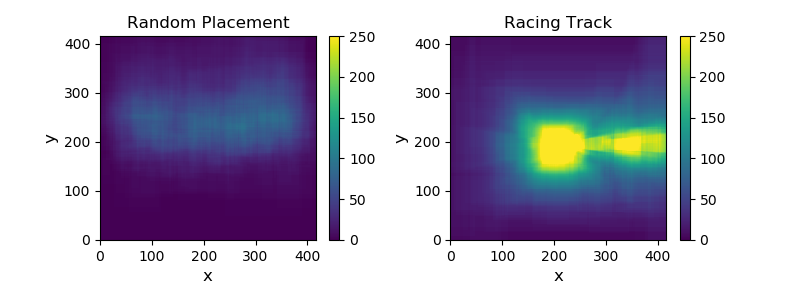
\includegraphics[width=\textwidth]{fig/heatmap_camplace}
			\caption{Heatmaps based on bounding boxes. Left the distribution when using random placement, right when moving through the scene with a drone motion model.}
			\label{fig:heatmap_camplace}
		\end{minipage}
		\begin{minipage}{\textwidth}
			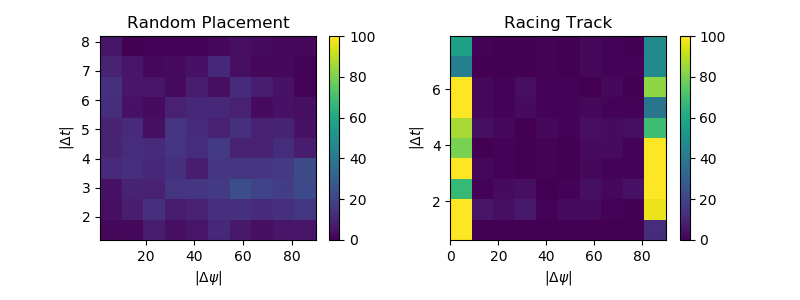
\includegraphics[width=\textwidth]{fig/hist2d_camplace}
			\caption{Histogram of Object Occurences in 3D coordinates.}
			\label{fig:hist2d_camplace}
		\end{minipage}
	\end{figure}
	
	\Cref{fig:heatmap_camplace} shows the distribution of bounding boxes when created with random camera placement and when following a racing track. It can be seen how with the drone motion model most of the objects are centered and distributed across the horizon. In contrast, the random placement leads to more evenly distributed object locations. While this plot shows where in the image the object appears, it does not include at which angle/distance the object appears.
	
	\Cref{fig:hist2d_camplace} shows a 2D histogram of the yaw angle of the object with respect to the camera as well as the distance. Thereby 0 corresponds to facing the object frontally, 180 degrees facing the object from the back. It is appearant how the random placement covers a much larger range of relative angles, while in the racing track certain angles do not appear at all. Even more importantly the largest bins of the racing track is an angle of 0 and a distance between 0m and 4m. These bins are almost not present when placing the camera randomly. This is because close to the camera the field of view is small, while the area of the object faced frontally is big. Hence, the probability of an object ending up at this specific location is relatively low. Furthermore, when placing the camera randomly there are no samples further away than 8m. This is because in the race track the camera traverses the room from one end where it can see almost all gates to another. The probability that the randomly placed camera ends up in a similar position is relatively low.
	
	\acp{CNN} are translation invariant by design but cannot inherently handle variation in rotation and scale. We hypothesize that the generation of samples with only one of the two methods misses important object appearances. Random placement does not cover most common appearances such as when flying through the racing gate. The drone motion model tends to limit object appearances depending on the flown trajectory as well as the created race court. 
	
	\subsection{Experiments}
	
	\subsubsection{Experiment - Context}
	
	\subsubsection{Experiment - View}
	
	
	In order to to evaluate this hypothesis two models are trained on 20 000 samples each. Model I is trained when placing the camera randomly, following the distribution in \Cref{eq:distroexp}. Model II is trained on varying racing courts. 
	
	For testing a dataset generated with a combination of both methods is used. That way it is ensured that similar view points as in the training sets are present. The dataset contains 1100 images and a total of XX objects. For random placement the distribution of \Cref{eq:distroexp} is used. The race court of the testset is different to the ones used for training. 
	
	\begin{figure}
		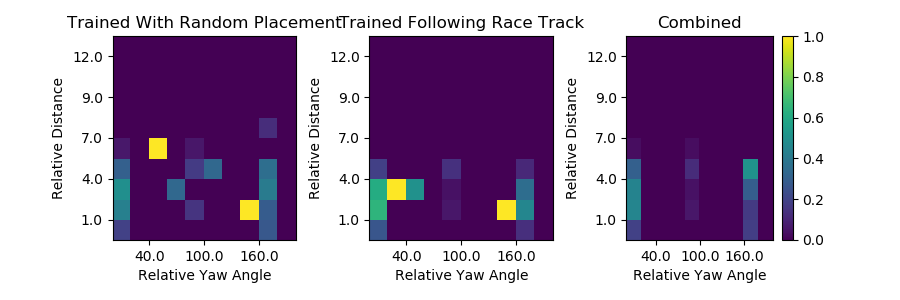
\includegraphics[width=\textwidth]{fig/recall_yaw}
		\caption{Performance across clusters.}
		\label{fig:recall_yaw}
	\end{figure}
	\begin{figure}
		\centering
		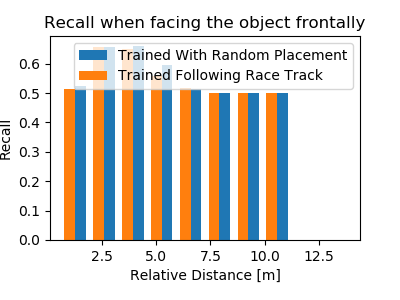
\includegraphics[width=0.5\textwidth]{fig/recall_front}
		\caption{Performance when facing the object frontally.}
		\label{fig:recall_front}
	\end{figure}
	
	
	\subsubsection{Results}
	
	
	\subsubsection{Discussion}
	
	\subsubsection{Conclusion}
	